\documentclass[a4paper, 10pt, twoside]{article}
\usepackage[left=2cm, right=2cm, top=2cm, bottom=3cm]{geometry}
\usepackage{amsmath}
\usepackage[shortlabels]{enumitem}
\usepackage{bbold}
\usepackage{cases}
\usepackage{systeme}
\usepackage{graphicx}

\begin{document}



\title{Algorithm Theory - Assignment 1}
\author{T\'eo Bouvard}
\maketitle

\section*{Problem 1}
In this problem, the objective is to maximize the profit of selling products X and Y, while satisfying production constraints on these products. The profit can be computed as

\begin{align*}
    profit & = revenue - cost                                                                              \\
           & = revenue - (time_{machine} \times cost_{machine} + time_{craftsman} \times cost_{craftsman})
\end{align*}

We can compute profits for each of the products

\begin{align*}
    profit(X) = 200 - (\frac{15}{60} \times 100 + \frac{20}{60} \times 20) = \frac{505}{3} \\
    profit(Y) = 300 - (\frac{20}{60} \times 100 + \frac{30}{60} \times 20) = \frac{770}{3}
\end{align*}

And formulate the problem as a linear programming problem. Let $a$ and $b$ be the number of products X and Y produced.

\begin{align*}
     & \text{maximize } a \times profit(X) + b \times profit(Y) \\
     & \text{subject to }
    \begin{cases}
        a \times time_{machine}(X) + b \times time_{machine}(Y) \le 40 \times 60     \\
        a \times time_{craftsman}(X) + b \times time_{craftsman}(Y) \le 35 \times 60 \\
        a \ge 10                                                                       \\
        a, b \ge 0                                                                   \\
    \end{cases}
\end{align*}

Which can be simplified as

\begin{align*}
     & \text{maximize } \frac{505}{3}a + \frac{770}{3}b \\
     & \text{subject to }
    \begin{cases}
        15 a + 20 b \le 2400 \\
        20 a + 30 b \le 2100 \\
        a \ge 10                             \\
        b \ge 0                              \\
    \end{cases}
\end{align*}

\section*{Problem 2}
\begin{enumerate}[a)]
    \item

          Let $x$ and $y$ be the number of products A and B produced. The problem can be formulated as such.

          \begin{align*}
               & \text{maximize } 3x + 5y \\
               & \text{subject to }
              \begin{cases}
                  12 x + 25 y \le 30 \times 60 \\
                  2 y - 5 x \ge 0              \\
                  x,y \ge 0                                 \\
              \end{cases}
          \end{align*}

          \begin{center}
              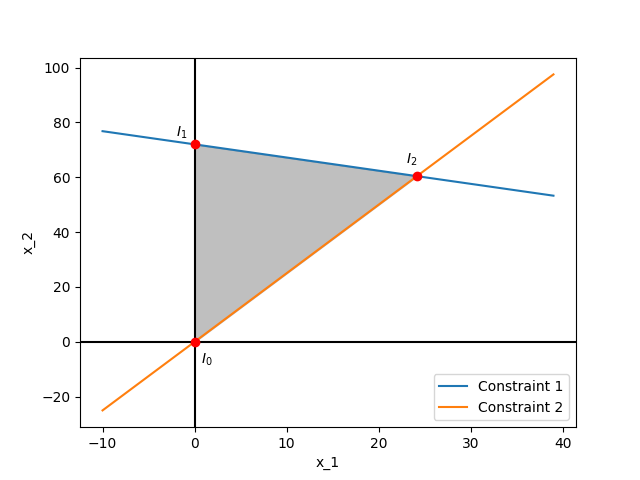
\includegraphics[width = .5 \textwidth]{graph1.png}
          \end{center}

          By graphing the feasible region, we see three candidate points. The first one $I_0 = (0, 0)$ can be trivially discarded as it leads to a profit of 0\$. Let's evaluate the objective function at the two other points. At $I_1 = (0, 72)$ the profit is 360\$. To compute the coordinates of the last point, we solve the following system of equations.

          \begin{align*}
            I_2 : 
              \systeme{
                  12 x + 25 y = 1800,
                  2 y - 5 x = 0
              }
              \implies
              \systeme{
                  \frac{149}{2}x = 1800,
                  y = \frac{5}{2} x
              }
              \implies
              \systeme{
                  x = \frac{3600}{149} \approx 24.2,
                  y = \frac{9000}{149} \approx 60.4
              }
          \end{align*}

          and at $I_2 = (24.2, 60.4)$ the profit is 374.5\$ which is the highest profit in this case. However, $x$ and $y$ are not integers. It is not specified in the exercise whether they should be or not, but as the problem is about a weekly production, we can assume that they do not need to be integer quantities because weeks are continuous. If we wanted to restrict the problem to an integer solution, we should pick $x = 24$ and $y = 60$, leading to a profit of 372\$.

    \item By doubling the production capacity without modifying the other constraints, the resulting profit is doubled. The company should then pay less than 374.5\$ for renting an extra machine in order to stay profitable. (Assuming integer values, the rent should not exceed 372\$).
\end{enumerate}

\section*{Problem 3}

\begin{enumerate}[a)]
    \item We want to minimize the total cost of transportation, while respecting constraints on the flights. This problem can be formulated as the following linear programming problem.
          Let $x$ and $y$ be the number of flights flown with aircrafts A and B respectively.

          \begin{align*}
               & \text{minimize } 10000x + 12000y \\
               & \text{subject to }
              \begin{cases}
                  30 x + 15 y \ge 300    \\
                  500 x + 750 y \ge 9000 \\
                  x + y \le 16                         \\
                  x, y \ge 0                           \\
              \end{cases}
          \end{align*}

          \begin{center}
              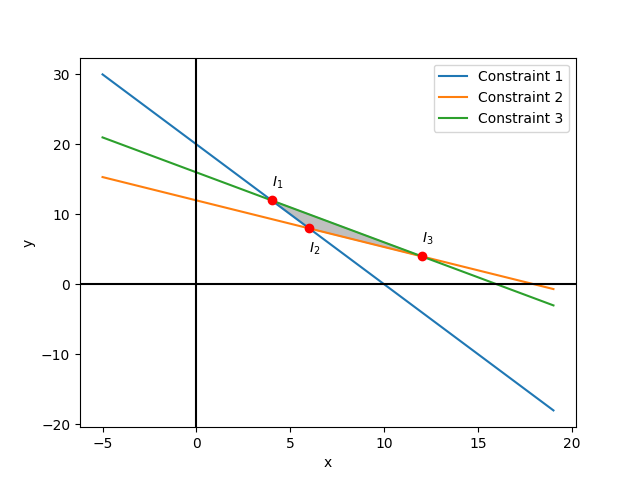
\includegraphics[width = .5\textwidth]{graph2.png}
          \end{center}

          With the graph method, we can identify the three points delimiting the feasible region. We first determine their coordinates, and then evaluate the objective function at these points.

          \begin{align*}
              I_1 :
              \systeme{
                  30x+15y=300,
                  x+y=16
              }
              \implies
              \systeme[.]{
                  x=4,
                  y=12
              }
              \implies \text{cost } = 184000\,\$ \\
              I_2 :
              \systeme{
                  30x+15y=300,
                  500x+750y=9000
              }
              \implies
              \systeme[.]{
                  x=6,
                  y=8
              }
              \implies \text{cost } = 156000\,\$ \\
              I_3 :
              \systeme{
                  x+y=16,
                  500x+750y=9000
              }
              \implies
              \systeme[.]{
                  x=12,
                  y=4
              }
              \implies \text{cost } = 168000\,\$ \\
          \end{align*}

          The lowest cost is achieved by using 6 flights with A and 8 flights with B, for a total cost of 156000\$.

\end{enumerate}

\section*{Problem 4}

\begin{enumerate}[a)]
    \item Graph method
          \begin{center}
              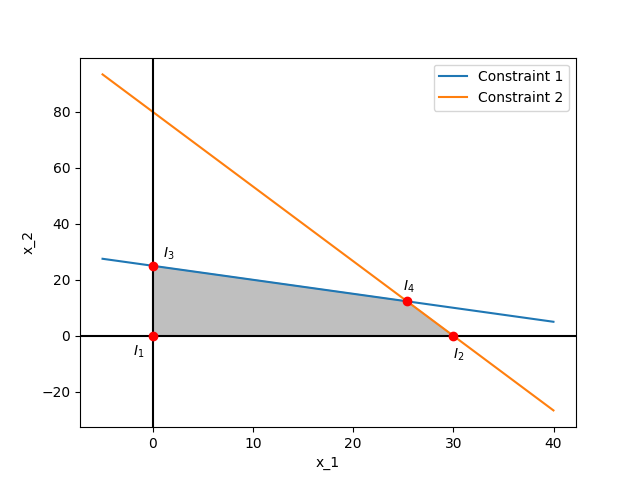
\includegraphics[width = .5 \textwidth]{graph3.png}
          \end{center}

          \begin{align*}
              I_1 :
              \systeme[]{
                  x_1 = 0,
                  x_2 = 0
              }
              \implies \text{objective } = 0                             \\
              I_2 :
              \systeme[]{
                  x_1 = 30,
                  x_2 = 0
              }
              \implies \text{objective } = 90                            \\
              I_3 :
              \systeme[]{
                  x_1 = 0,
                  x_2 = 25
              }
              \implies \text{objective } = 125                           \\
              I_4 :
              \systeme{
                  x_1+2x_2=50,
                  8x_1+3x_2=240
              }
              \implies
              \systeme[]{
                  x_1 = \frac{330}{13},
                  x_2 = \frac{160}{13}
              }
              \implies \text{objective } = \frac{1790}{13} \approx 137.7 \\
          \end{align*}

    \item Simplex algorithm

          We first convert the linear problem to its the slack form by introducing two slack variables $s_1$ and $s_2$.

          \begin{align*}
               & \text{maximize } z = 3x_1 + 5x_2 \\
               & \text{subject to }
              \begin{cases}
                  s_1 = 50 - x_1 - 2x_2    \\
                  s_2 = 240 - 8x_1 - 3x_2  \\
                  x_1, x_2, s_1, s_2 \ge 0 \\
              \end{cases}
          \end{align*}

          A basic feasible solution is $(x_1, x_2, s_1, s_2) = (0, 0, 50, 240)$. However, this solution is not optimal as the objective function can be improved by picking a greater $x_1$ or $x_2$. To do the first pivot, we choose $x_2$ as the entering variable because it has the highest coefficient in the objective function. To choose the leaving variable, we find the tightest constraint on $x_2$. In the first constraint, $x_2$ is limited to 25, and in the second constraint it is limited to 80. Thus the leaving variable is $s_1$, and we rewrite the problem with $x_2 = 25 - \frac{x_1}{2} - \frac{s_1}{2}$

          \begin{align*}
               & \text{maximize } z = 125 + \frac{x_1}{2} - \frac{5}{2}s_1 \\
               & \text{subject to }s
              \begin{cases}
                  x_2 = 25 - \frac{x_1}{2} - \frac{s_1}{2}     \\
                  s_2 = 165 - \frac{13}{2}x_1 + \frac{3}{2}s_1 \\
                  x_1, x_2, s_1, s_2 \ge 0                     \\
              \end{cases}
          \end{align*}

          The only remaining entering variable able to increase the objective function is $x_1$. Constraint 1 limits it to 50 and constraint 2 limits it to $\frac{330}{13} \approx 25.4$. The second constraint being tighter than the first, we choose $s_2$ as leaving variable and rewrite the problem with $x_1=\frac{330}{13}+\frac{3}{10}s_1-\frac{2}{13}s_2$

          \begin{align*}
               & \text{maximize } z = \frac{1790}{13} - \frac{47}{20}s_1 - \frac{1}{26}s_2 \\
               & \text{subject to }s
              \begin{cases}
                  x_2 = \frac{160}{13}-\frac{8}{13}s_1+\frac{1}{13}s_2 \\
                  x_1=\frac{330}{13}+\frac{3}{10}s_1-\frac{2}{13}s_2   \\
                  x_1, x_2, s_1, s_2 \ge 0                             \\
              \end{cases}
          \end{align*}

          At this stage, the basic feasible solution of the objective function cannot be increased further because there is only substractions of positive terms after the first constant term. Therefore, the optimal solution is $z = \frac{1790}{13} \approx 137.7$, obtained for the variables $x_1 = \frac{330}{13}$ and $x_2 = \frac{160}{13}$.

    \item Programming method

          Not wanting to run proprietary software, this problem was solved using GNU's GLPK.
          This first image shows the program used.
          \begin{center}
              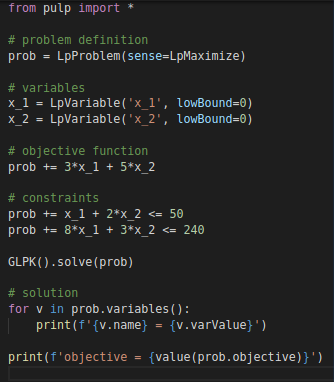
\includegraphics[width = .5 \textwidth]{linprog_script.png}
          \end{center}
          This second image shows the output of the execution.
          \begin{center}
            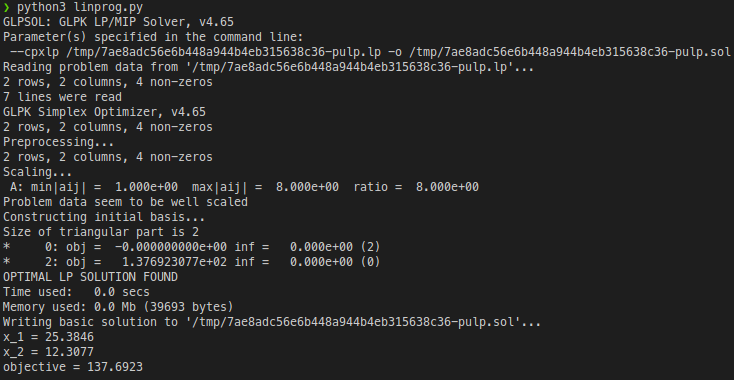
\includegraphics[width = .5 \textwidth]{linprog_run.png}
          \end{center}

    We can see that we get the same results with the three techniques. The optimal setting of variables to maximize the objective function is $x_1 = \frac{330}{13} \approx 25.4$ and $x_2 = \frac{160}{13} \approx 12.3$, for an objective value of $z = \frac{1790}{13} \approx 137.7.$
\end{enumerate}

\end{document}
